\chapter{Fermionische Vorzeichen und supersymmetrische Auslöschungen}

\lectureoverview{Supersymmetrie verknüpft Bosonen mit Fermionen. Warum man eine solche Beziehung anstrebt, lässt sich jedoch leichter erkennen, bevor man ihre Algebra formuliert. Wir beginnen mit der Topologie von Drehungen, machen das Vorzeichen der Fermionen-Wellenfunktion durch Interferenz beobachtbar, leiten das Minuszeichen einer geschlossenen Fermionschleife aus der Antisymmetrie beim Teilchenaustausch her und nutzen dann die entgegengesetzten Vorzeichen bosonischer und fermionischer Schleifen, um Auslöschungen der Vakuumenergie und der skalaren Selbstenergie zu motivieren. In der zweiten Hälfte geht es darum, wie stark Supersymmetrie gebrochen sein darf, wie man Superpartner nachweisen könnte und warum exakte Supersymmetrie die gewöhnliche Schalenstruktur der Atome aufheben würde.}

\section{Vor der Supersymmetrie: eine Besonderheit von Drehungen}

Supersymmetrie ist eine Symmetrie zwischen Fermionen und Bosonen. Bevor wir versuchen, sie zu konstruieren, lohnt es sich jedoch, sich daran zu erinnern, wie unterschiedlich diese beiden Teilchenarten auf Drehungen reagieren. Diese Frage beginnt mit einer topologischen Tatsache, die sich leicht vorführen lässt und die man erstaunlich schwer wieder vergisst, wenn man sie einmal gesehen hat.

Halte eine Hand mit der Handfläche nach oben und drehe das Handgelenk um \(2\pi\). Die Hand kehrt in ihre ursprüngliche Ausrichtung zurück, doch der Arm befindet sich offensichtlich nicht wieder in einer gleichwertigen Konfiguration: Er ist verdreht. Dreht man ihn um weitere \(2\pi\) und bewegt dabei den Arm nach Bedarf, lässt sich die Verdrehung lösen. Eine Drehung um \(2\pi\) lässt sich also bei festgehaltener Umgebung nicht stetig in keine Drehung überführen, eine Drehung um \(4\pi\) dagegen schon. Die Vorführung mit der Hand ist im wörtlichsten Sinn ein Beweis durch Handwedeln.

Dasselbe lässt sich ohne Bezug auf die Anatomie zeigen. Lege eine Kugel in einen feststehenden Kasten und verbinde sie mit beliebig vielen biegsamen, dehnbaren, aber unzerreißbaren Schnüren mit den Wänden. Drehe die Kugel einmal um \(2\pi\). Die Schnüre verheddern sich, und keine Bewegung der Schnüre allein stellt die ursprüngliche Konfiguration wieder her. Dreht man die Kugel insgesamt um den Winkel \(4\pi\), können die Schnüre um sie herumgeführt werden, bis sich das Knäuel auflöst. Die Wände stehen für das räumliche Unendliche: Der Vergleich ist nur sinnvoll, weil der Rand nicht zusammen mit der Kugel gedreht wird.

\begin{classroomqa}
\audiencequestion{Könnte man das Knäuel lösen, indem man den Kasten dreht? \lecturetimestamp{00:02:53}}
\lecturerresponse{Damit ändert sich das Problem. Der Kasten steht für das räumliche Unendliche und bleibt fest. Wir vergleichen eine Drehung des Objekts relativ zu seiner Umgebung, nicht eine gemeinsame Drehung von Objekt und Umgebung.}
\end{classroomqa}

\begin{classroomqa}
\audiencequestion{Warum dreht man die Kugel nicht einfach noch einmal um \(2\pi\)? \lecturetimestamp{00:03:20}}
\lecturerresponse{Genau darin besteht der Unterschied zwischen den beiden Fällen. Ohne die Kugel weiterzudrehen, lässt sich das Knäuel nach einer Drehung um \(2\pi\) nicht lösen. Nach der zweiten Drehung, also insgesamt \(4\pi\), ist das möglich.}
\end{classroomqa}

In der modernen Sprache der Gruppentheorie hat die Drehgruppe zwei topologische Klassen geschlossener Wege:
\begin{equation}
\pi_1\!\left(SO(3)\right)\cong \mathbb Z_2.
\end{equation}
Einmaliges Durchlaufen ist nichttrivial, zweimaliges dagegen gehört zur trivialen Klasse.
Äquivalent dazu ist \(SU(2)\) eine zweifache Überlagerung von \(SO(3)\). Hier liegt der geometrische Ursprung des Fermionenvorzeichens.

\editorialnote{Die Sprache von \(SO(3)\), \(SU(2)\) und der Fundamentalgruppe macht die Topologie explizit. Die Vorführung mit dem Arm und die mit den Schnüren zeigen geometrisch dasselbe zweifache Verhalten.}

\section{Was eine Drehung um \texorpdfstring{\(2\pi\)}{2 pi} mit einem Quantenzustand macht}

Fixieren wir nun die Position eines Teilchens und betrachten nur seinen Spinzustand, bezeichnet mit \(\ket{\psi}\). Teilchen mit ganzzahligem Spin sind Bosonen, Teilchen mit halbzahligem Spin Fermionen. Eine physikalische Drehung lässt sich realisieren, indem man den Spin eines geladenen Teilchens in ein starkes Magnetfeld bringt und das Feld dreht, oder indem man den Spin in einem festen Feld um den gewünschten Winkel präzedieren lässt.

\begin{classroomqa}
\audiencequestion{Wie lässt sich der Spin eines Elektrons im Labor tatsächlich drehen? \lecturetimestamp{00:05:26}}
\lecturerresponse{Ein Magnetfeld dient dazu als Stellgröße. Man kann ein ausreichend starkes Feld drehen, sodass der Spin ihm folgt, oder den Spin um ein festes Feld präzedieren lassen. Das Elektron mit der Hand zu greifen, ist keine konkurrenzfähige Versuchsmethode.}
\end{classroomqa}

Angenommen, eine volle Drehung um \(2\pi\) multipliziert den Zustand mit einer Phase:
\begin{equation}
R(2\pi)\ket{\psi}=\xi\ket{\psi}.
\end{equation}
Wendet man die Operation zweimal an, ergibt sich
\begin{equation}
R(4\pi)\ket{\psi}=\xi^2\ket{\psi}.
\end{equation}
Da der Weg über \(4\pi\) topologisch trivial ist, muss er in diesem Vergleich wie die Identität wirken. Folglich gilt
\begin{equation}
\xi^2=1,
\qquad
\xi=+1\ \hbox{or}\ -1.
\end{equation}
Bosonen entsprechen dem Pluszeichen, Fermionen dem Minuszeichen:
\begin{align}
R(2\pi)\ket{\psi_B}&=+\ket{\psi_B},\\
R(2\pi)\ket{\psi_F}&=-\ket{\psi_F}.
\end{align}
Für einen Zustand mit festem Spin \(j\) lässt sich dies kompakt so ausdrücken:
\begin{equation}
R(2\pi)=(-1)^{2j}.
\end{equation}
Im Transkript heißt es kurz, die zweite Möglichkeit entspreche einer Multiplikation mit \(2\pi\); aus der Herleitung im Kontext und dem Tafelargument geht jedoch klar hervor, dass der gemeinte Faktor \(-1\) ist.

Zunächst scheint das physikalisch bedeutungslos. Wenn sich das Vorzeichen der gesamten Wellenfunktion ändert,
\begin{equation}
\Psi\longmapsto-\Psi,
\end{equation}
bleiben die Wahrscheinlichkeiten unverändert, denn
\begin{equation}
(-\Psi)^*(-\Psi)=\Psi^*\Psi.
\end{equation}
Man betrachte zwei Ensembles identisch präparierter Elektronen. Dreht man jedes Teilchen des einen Ensembles um \(2\pi\) und lässt das andere unverändert, kann keine Messung an einem isolierten Teilchen verraten, aus welchem Ensemble es stammt. Eine globale Phase ist keine Observable.

\section{Das Minuszeichen relativ machen}

Das Vorzeichen wird beobachtbar, wenn es auf einen kohärenten Zweig einer Wellenfunktion wirkt, aber nicht auf den anderen. Schicke Elektronen einzeln durch einen Zweiwegeapparat. Bestimme nicht, welchen Weg sie nehmen, denn die Weginformation zerstört die Interferenz. Die Amplituden für den oberen und den unteren Weg seien \(\psi_1\) und \(\psi_2\); der wieder zusammengeführte Zustand lautet dann
\begin{equation}
\Psi=\psi_1+\psi_2.
\end{equation}
Stellen wir uns vorübergehend vor, jeder Zweig werde in einem magnetischen Bereich eingeschlossen. Drehe das Feld, das zum zweiten Zweig gehört, allein um \(2\pi\). Ist das Teilchen ein Fermion, wird der Zustand zu
\begin{equation}
\Psi'=\psi_1-\psi_2.
\end{equation}
Das ist kein globales Vorzeichen mehr. Die relative Phase verschiebt Interferenzmaxima zu Minima. Sind die beiden zurückkehrenden Wellenpakete Spiegelbilder bezüglich der Detektormitte, verschwindet die antisymmetrische Kombination im Zentrum:
\begin{equation}
\Psi'(0)=\psi_1(0)-\psi_2(0)=0.
\end{equation}
Das Elektron wird daher an diesem Symmetriepunkt niemals nachgewiesen. Eine Drehung beider Zweige würde stattdessen \(-\psi_1-\psi_2=-\Psi\) ergeben, was keinen beobachtbaren Effekt hat.

In der Vorlesung wird der relationale Charakter des Experiments betont. Einen Magnetbereich relativ zum anderen zu drehen, entspricht der Drehung der Kugel bei festgehaltenem Kasten. Beide Bereiche gemeinsam zu drehen, entspricht der gemeinsamen Drehung von Kugel und Kasten. Eine relative Drehung um \(4\pi\) hebt den Effekt auf, weil der Fermionenzustand dabei mit einem Pluszeichen zurückkehrt. Das Experiment wurde 1967 von Yakir Aharonov und Leonard Susskind vorgeschlagen und später in interferometrischer Form realisiert, wie nebenbei in der Vorlesung erwähnt wird. Dasselbe Prinzip lässt sich auf Elektronen oder geladene Ionen anwenden: Ein verschobenes Streifenmuster weist auf einen halbzahligen Spin hin, ein unverändertes auf einen ganzzahligen.

\begin{classroomqa}
\audiencequestion{Kehrt das verschobene Muster zum ursprünglichen zurück, wenn das relative Feld um \(4\pi\) gedreht wird? \lecturetimestamp{00:12:21}}
\lecturerresponse{Ja. Zwei Vorzeichenänderungen ergeben zusammen \(+1\), sodass die für den Austausch von Maxima und Minima verantwortliche relative Phase verschwindet.}
\end{classroomqa}

\begin{classroomqa}
\audiencequestion{Wie wörtlich sind die Schnüre im Kasten einem Fermion zuzuordnen? \lecturetimestamp{00:13:43}}
\lecturerresponse{Sie sind eine topologische Gedächtnisstütze, keine physikalischen Schnüre, die an einem Elektron befestigt wären. Ein Boson verhält sich so, als hinterließe eine Drehung um \(2\pi\) keine Erinnerung; ein Fermion behält genau die Vorzeichen-Erinnerung, die durch das nichttriviale Knäuel dargestellt wird.}
\end{classroomqa}

\begin{classroomqa}
\audiencequestion{Befinden sich in den beiden Magnetbereichen zwei Elektronen, von denen eines gedreht wird und das andere nicht? \lecturetimestamp{00:14:29}}
\lecturerresponse{Nein. Es handelt sich um ein Elektron in einer kohärenten räumlichen Superposition. Es besitzt eine Amplitude, sich in jedem der beiden Zweige aufzuhalten, und der Apparat darf nicht erkennen lassen, in welchem Zweig es sich befand. Die Drehung eines Bereichs verändert eine Amplitude relativ zur anderen; die Drehung beider ändert nur die gemeinsame Phase.}
\end{classroomqa}

Der Winkel \(2\pi\) ist besonders, weil die Spinorientierung zu sich selbst zurückkehrt, während der Spinor ein Vorzeichen annimmt. Eine beliebige relative Drehung verändert auch die Spinorientierung. Kehren die beiden Wegzustände mit den Spinzuständen \(\ket{\chi_1}\) und \(\ket{\chi_2}\) zurück, ist der Interferenzterm proportional zu
\begin{equation}
\braket{\chi_1}{\chi_2}.
\end{equation}
Sein Betrag bestimmt die Sichtbarkeit der Streifen.\editorialnote{Die Formel für die Spinüberlappung ist eine übliche Ergänzung zur qualitativen Diskussion der Vorlesung über teilweise und vollständige Interferenzverluste.} Orthogonale Spinzustände enthalten perfekte Weginformation und interferieren nicht.

\begin{classroomqa}
\audiencequestion{Was geschieht, wenn man misst, in welchem Magnetbereich sich das Elektron befand? \lecturetimestamp{00:18:03}}
\lecturerresponse{Das Interferenzmuster wird zerstört. Jede Aufzeichnung, die die beiden Wege unterscheidet, verhindert die kohärente Addition ihrer Amplituden.}
\end{classroomqa}

\begin{classroomqa}
\audiencequestion{Wenn alle Spins anfangs dieselbe Richtung haben und der Endspin gemessen wird, ändert die Operation \(2\pi\) dann selbst diese Richtung? \lecturetimestamp{00:18:17}}
\lecturerresponse{Nein. Nach \(2\pi\) ist die physikalische Spinrichtung dieselbe; lediglich der fermionische Zweig hat ein Minuszeichen erhalten. Deshalb kann diese Operation die Interferenz verändern, ohne eine andere Spinorientierung als Wegmarkierung zu hinterlassen.}
\end{classroomqa}

\begin{classroomqa}
\audiencequestion{Was geschieht, wenn das Feld nur um \(\pi\) statt um \(2\pi\) gedreht wird? \lecturetimestamp{00:18:43}}
\lecturerresponse{Dann ändert sich die Spinrichtung. Ein Zweig mit Spin nach oben und einer mit Spin nach unten sind unterscheidbar und können nicht interferieren. Bei Zwischenwinkeln nimmt die Sichtbarkeit stetig ab; eine relative Drehung um \(180^\circ\) zerstört sie vollständig.}
\end{classroomqa}

\section{Austauschsymmetrie und das Vorzeichen einer geschlossenen Schleife}

Die Diskussion der Drehungen hat ein fermionisches Minuszeichen herausgearbeitet. Ein zweites, eng damit verwandtes Vorzeichen tritt beim Austausch identischer Teilchen auf. Für eine Zweiteilchen-Wellenfunktion gilt
\begin{align}
P_{12}\Psi_B(1,2)&=+\Psi_B(1,2)=+\Psi_B(2,1),\\
P_{12}\Psi_F(1,2)&=-\Psi_F(1,2)=-\Psi_F(2,1).
\end{align}
Bosonische Zustände sind symmetrisch, fermionische antisymmetrisch.

\begin{figure}[htbp]
\centering
\includegraphics[width=0.74\textwidth]{lecture_02_figure_02.png}
\lectureframe{00:24:27}
\caption{Das Austauschargument in der Zustandsnotation. Im Bild ist nur die Beschriftung des Ket-Zustands sicher lesbar; die Antisymmetriegleichungen sind im Text gesetzt und werden nicht der verdeckten Kreidebeschriftung zugeschrieben.}
\end{figure}

Nun können wir das relative Vorzeichen einer geschlossenen Teilchenschleife bestimmen, ohne ihr Integral auszuwerten. Betrachte ein Vakuum-Feynman-Diagramm ohne äußere Beine. Man kann es sich als Teilchen vorstellen, das eine geschlossene Bahn durch die Raumzeit verfolgt, oder als Teilchen-Antiteilchen-Paar, das erzeugt und später wieder vernichtet wird. Ein solches Vakuumdiagramm trägt zur Vakuumamplitude und damit zur Vakuumenergie bei.

Beginnen wir mit zwei voneinander getrennten Kopien der Schleife. Getrennte Diagramme multiplizieren sich. Hat eine Schleife das Vorzeichen \(\sigma\), hat das Paar das Vorzeichen
\begin{equation}
\sigma^2=+1.
\end{equation}
Schneide beide Schleifen zu einem gemeinsamen Zeitpunkt auf, etwa bei \(t=0\). An diesem Schnitt liegen zwei identische Teilchen vor. Verbindet man sie ohne Austausch erneut, erhält man wieder die beiden getrennten Schleifen. Vertauscht man die beiden Teilchen vor dem erneuten Verbinden, entsteht topologisch eine einzige Schleife. Der Austausch liefert für Bosonen den Faktor \(+1\) und für Fermionen \(-1\). Da das Vorzeichen des anfänglichen Schleifenpaars positiv war, ergeben sich für die Schleife die Vorzeichen
\begin{equation}
\begin{aligned}
\operatorname{sign}(\text{closed boson loop})&=+1,\\
\operatorname{sign}(\text{closed fermion loop})&=-1.
\end{aligned}
\end{equation}
Allgemeiner trägt ein Diagramm mit \(L_F\) unabhängigen geschlossenen Fermionschleifen den Faktor
\begin{equation}
(-1)^{L_F}.
\end{equation}
Die Vorlesung leitet diese Regel bewusst aus dem Austausch her, statt sich auf Grassmann-Integration zu berufen. Das elementare Argument macht den physikalischen Ursprung des Vorzeichens sichtbar.

\section{Entgegengesetzte Schleifenvorzeichen und Vakuumenergie}

Eine bosonische Vakuumschleife erhöht den Vakuumbeitrag mit einem Vorzeichen, während eine fermionische Schleife mit dem entgegengesetzten Vorzeichen eingeht. Das liegt nahe, denn die beobachtete Dichte der Dunklen Energie ist im Vergleich zu naiven Abschätzungen mit einem Abschneideparameter in der Quantenfeldtheorie außerordentlich klein. Die Vorlesung beziffert die berüchtigte Abweichung auf ungefähr \(123\) Größenordnungen. Der genaue Exponent hängt davon ab, welche ultraviolette Skala man zugrunde legt; entscheidend ist die gewaltige Diskrepanz.

Der Wert einer Schleife hängt von mehr als der Statistik ab. Er hängt von Masse, Ladung, Multiplizität und Wechselwirkungen ab. Stimmen jedoch ein Boson und ein Fermion in allen relevanten Eigenschaften überein, können sich ihre gleich großen Beiträge aufheben:
\begin{equation}
\begin{gathered}
m_B=m_F,\qquad q_B=q_F,\qquad g_B=g_F,\\
\Delta\rho_{\mathrm{vac}}^{(B)}
+\Delta\rho_{\mathrm{vac}}^{(F)}=0.
\end{gathered}
\end{equation}
Diese Beobachtung löst das Problem der kosmologischen Konstanten nicht. Sie liefert lediglich etwas, das gewöhnliche bosonische Schleifen allein nicht liefern könnten: Beiträge mit entgegengesetztem Vorzeichen. In einer exakt ungebrochenen global supersymmetrischen Theorie können sich die Vakuumenergien unter den entsprechenden Voraussetzungen tatsächlich exakt aufheben; nach dem Bruch der Supersymmetrie bleibt der beobachtete kleine, aber von null verschiedene Wert unerklärt.\editorialnote{Diese Einschränkung grenzt die Motivation der Vorlesung vom wesentlich schwierigeren Problem der kosmologischen Konstanten ab.}

Dass exakt übereinstimmende Partner die Natur beschreiben, ist bereits widerlegt. Hätte das Elektron einen Spin-null-Partner mit derselben Masse und elektrischen Ladung, könnte die Elektron-Positron-Annihilation über ein virtuelles Photon ein Paar solcher Teilchen erzeugen:
\begin{equation}
e^-e^+\longrightarrow\gamma^*
\longrightarrow\widetilde e^-\widetilde e^+.
\end{equation}
Ein entartetes geladenes Skalarteilchen wäre den gewöhnlichen Beschleunigerexperimenten nicht entgangen. Die Spiegelung von Bosonen auf Fermionen kann daher keine exakte Symmetrie des beobachteten Spektrums sein. Gemeint ist eine Spiegelung zwischen Teilchentypen, nicht im physikalischen Raum.

\section{Das unmittelbarere Ziel: die skalare Selbstenergie}

Die Vakuumenergie ist das erste Beispiel, doch im Mittelpunkt der Vorlesung steht die radiative Instabilität skalarer Massen. Ein Skalarteilchen, dessen nackte Masse null ist, kann eine quadratisch von der Abschneideskala abhängige Korrektur erhalten. Schematisch gilt
\begin{equation}
\Delta m_H^2\sim \frac{g_B^2}{16\pi^2}\Lambda^2
\end{equation}
für eine bosonische Schleife. Fermionmassen sind anders geschützt: Besitzt ein masseloses Fermion eine exakte chirale Symmetrie, können radiative Korrekturen keinen additiven Massenterm erzeugen. Das war das Links-rechts-Argument der vorherigen Vorlesung.

Stellen wir uns nun eine Symmetrie vor, die stark genug ist, ein Skalar- und ein Fermionfeld in ein und dasselbe Multiplett zu stellen und ihre Wechselwirkungen aufeinander abzustimmen. Dann tritt eine Fermionschleife mit dem entgegengesetzten Vorzeichen auf:
\begin{equation}
\Delta m_H^2
\sim
\frac{g_B^2-g_F^2}{16\pi^2}\Lambda^2+\cdots .
\end{equation}
Erzwingt die Supersymmetrie \(g_B=g_F\) und gleiche Massen, heben sich die quadratischen Terme auf. Der Schutz des Fermions wird so auf seinen bosonischen Partner übertragen. Das ist nicht bloß ein numerischer Zufall zwischen zwei Diagrammen; die Symmetrie muss die Auslöschung in jeder Ordnung und für jede zulässige Wechselwirkung erzwingen.

Der großflächige Tafelvergleich zeigt, wie die Vorlesung von einzelnen Schleifen zu gepaarten Schleifenkorrekturen propagierender Teilchen übergeht.

\begin{figure}[htbp]
\centering
\includegraphics[width=0.79\textwidth]{lecture_02_figure_04.png}
\lectureframe{00:40:23}

\medskip
\begin{tikzpicture}[scale=0.9]
\draw (-4.2,0) circle (0.55);
\draw[dashed] (-2.4,0) circle (0.55);
\draw (0,0) -- (3.7,0);
\fill (1.85,0) circle (0.055);
\draw (1.85,0) -- (1.85,0.25);
\draw[dashed] (1.85,0.85) circle (0.6);
\end{tikzpicture}
\caption{Ein großflächiger Vergleich gewöhnlicher Schleifentopologien mit denen der Partnerteilchen. Die gesetzte Skizze gibt nur den sichtbaren topologischen Unterschied wieder; verdeckte Teilchenbeschriftungen werden nicht ergänzt.}
\end{figure}

Nach der Pause im Hörsaal setzt das Argument mit dem sogenannten Bild nullter Ordnung neu an. Damit ist keine Ordnung der Störungstheorie gemeint, sondern die einfachste brauchbare Darstellung:
\begin{quote}
Zu jedem Teilchen gibt es einen Superpartner mit entgegengesetzter Statistik. Jedes Fermion hat einen bosonischen Partner und jedes Boson einen fermionischen Partner.
\end{quote}
In einer exakten supersymmetrischen Theorie wären die Partner außerdem entartet, also gleich schwer. Die Natur ist nicht auf diese Weise entartet. Sind die Massen jedoch verschieden, aber nicht allzu weit voneinander entfernt, kann die Auslöschung immer noch gut genug sein, um eine explosionsartig große skalare Korrektur zu verhindern. Bei weicher Supersymmetriebrechung wird die gefährliche Skala schematisch durch die Aufspaltung der Superpartner ersetzt:
\begin{equation}
\Delta m_H^2\sim
\frac{g^2}{16\pi^2}\,\Delta m_{\mathrm{SUSY}}^2
\ln\!\frac{\Lambda^2}{\Delta m_{\mathrm{SUSY}}^2}
\end{equation}
bis auf modellabhängige Koeffizienten.\editorialnote{Diese Formel drückt die qualitative Aussage der Vorlesung aus: Bei unvollständiger Massenübereinstimmung bleibt eine Restkorrektur, die von der Aufspaltung bestimmt wird; sie ist nicht von der Tafel abgeschrieben.}

\section{Gebrochene Supersymmetrie und die experimentelle Wette von 2010}

Zum Zeitpunkt der Aufzeichnung dieser Vorlesung, im Jahr 2010, war noch kein Superpartner beobachtet worden. Die unmittelbare Schlussfolgerung lautete, dass die Partner, falls es sie gibt, schwerer als die bekannten Teilchen sein und die Reichweite früherer Maschinen übersteigen müssen. In supersymmetrischen Modellen unterscheidet man außerdem Teilchen, deren Massen erst nach der elektroschwachen Symmetriebrechung entstehen, von Zuständen, die auch größere, symmetrieerhaltende Massen haben dürfen. Die Vorlesung führt dies als Begründung dafür an, warum die sichtbare Hälfte eines supersymmetrischen Spektrums leicht und die unentdeckte Hälfte schwerer sein könnte, bezeichnet diese Konstellation aber offen als gewagt. Susskind äußert seine eigene Erwartung, Superpartner würden entdeckt, und kennzeichnet sie unmittelbar darauf als Vermutung und nicht als Ergebnis.

Der Large Hadron Collider stand daher im Mittelpunkt des Ausblicks der Vorlesung. Von ihm erwartete man die Suche sowohl nach dem Higgs-Boson als auch nach Superpartnern. Diese Aussagen sind vor dem Hintergrund des Jahres 2010 zu verstehen: Die Vorlesung erläutert die experimentelle Wette vor der Entdeckung des Higgs-Bosons und vor den späteren Suchergebnissen des LHC.

Warum sollte ein durch Natürlichkeit motivierter Superpartner nicht auf der Planck-Skala liegen? Weil er dann die ihm zugedachte Aufgabe verfehlen würde. Unterscheiden sich die Massen von Boson und Fermion enorm, heben sich ihre Schleifenintegrale oberhalb der leichteren Masse nicht mehr auf. Die verbleibende skalare Korrektur wird grob durch die große Massendifferenz und nicht durch die elektroschwache Skala bestimmt. Supersymmetrie auf einer beliebig weit entfernten Skala bleibt zwar eine mathematische Symmetrie, liefert aber keine überzeugende Erklärung mehr für einen leichten Higgssektor.

Die Vorlesung übersetzt dies in die damalige Erwartung, die relevanten Massendifferenzen sollten höchstens einige hundert GeV betragen und daher in Reichweite des LHC liegen. Diese zahlenmäßige Abschätzung ist historisch und modellabhängig; wichtiger ist die logische Kette:
\begin{equation}
\begin{gathered}
\text{Higgs protection}\\
\Downarrow\\
\text{effective boson--fermion cancellation}\\
\Downarrow\\
\Delta m_{\mathrm{SUSY}}\ \text{not too large}.
\end{gathered}
\end{equation}

\begin{classroomqa}
\audiencequestion{Könnten sich fermionische Beiträge nicht einfach insgesamt mit allen bosonischen Beiträgen aufheben, ohne dass es paarweise Partner gibt? \lecturetimestamp{00:45:01}}
\lecturerresponse{Sie könnten sich numerisch aufheben, doch das wäre eine zufällige Auslöschung, die ebenso fein abgestimmt wäre wie das ursprüngliche Problem. Der Vorschlag der Supersymmetrie geht weiter: Plausible Postulate erzwingen aufeinander abgestimmte Beiträge, während gebrochene Supersymmetrie erklärt, warum die Massen nur näherungsweise übereinstimmen. Die Vakuumenergie diente als Beispiel; hier geht es unmittelbar um die Selbstenergie des Higgs-Bosons.}
\end{classroomqa}

\begin{classroomqa}
\audiencequestion{Setzt die Bezeichnung einer solchen Gesamtauslöschung als unnatürlich bereits eine reduktionistische Art voraus, die Theorie zu ordnen? \lecturetimestamp{00:47:51}}
\lecturerresponse{Das ist ein berechtigter Einwand. Niemand verfügt über eine endgültige Definition von Natürlichkeit, und die Suche besteht zum Teil darin, tastend nach einer überzeugenden Erklärung zu suchen. Supersymmetrie und spontane Supersymmetriebrechung bieten bekannte mathematische Rahmen, die das gewünschte Muster erzwingen können. Offen bleibt, ob die Natur diesen Rahmen nutzt und ob er eindeutig ist.}
\end{classroomqa}

\section{Direkte Erzeugung, virtuelle Effekte und Zerfallskaskaden}

Ein schweres Teilchen muss nicht on shell erzeugt werden, um ein Experiment zu beeinflussen. Es kann virtuell in einer Schleife auftreten und eine gewöhnliche Elektron-Positron-Streuamplitude geringfügig verändern. Präzisionsmessungen der elektroschwachen Wechselwirkungen schränken Superpartner daher auch dann ein, wenn die Schwerpunktsenergie unterhalb der Schwelle für ihre direkte Paarerzeugung liegt:
\begin{equation}
\sqrt{s}<2m_{\widetilde p}.
\end{equation}Die Einschätzung der Vorlesung aus dem Jahr 2010 lautet, dass Präzisionsdaten den Parameterraum der Supersymmetrie bereits einengten, sie aber noch nicht ausgeschlossen hatten.

\begin{classroomqa}
\audiencequestion{Könnte man Superpartner indirekt erschließen, so wie frühere schwere Teilchen anhand präziser Produktionsraten eingeschränkt wurden, bevor sie direkt beobachtet wurden? \lecturetimestamp{00:49:01}}
\lecturerresponse{Ja. Eine virtuelle Superpartnerschleife verändert eine gewöhnliche Amplitude geringfügig; damit wird das Problem zu einer Präzisionsuntersuchung der elektroschwachen Phänomenologie und nicht zu einer Frage direkter Erzeugung. Besonders hilfreich wäre ein sauberer Elektron-Positron-Beschleuniger mit ausreichend hoher Energie. Protonenkollisionen sind komplizierter, weil ein Proton ein zusammengesetzter Zustand aus Quarks und Gluonen ist: Tatsächlich kollidieren fluktuierende Bestandteile und nicht zwei Elementarteilchen mit genau bekannten Anfangsbedingungen.}
\end{classroomqa}

Ein Student fragt, ob sich die Reaktion auch umgekehrt abspielen ließe, wenn man mit reichlich vorhandenen Superteilchen beginnt. Das Hindernis ist nicht die Zeitumkehrsymmetrie, sondern die Verfügbarkeit. Schwere Superpartner müssen zunächst erzeugt werden, und die meisten zerfallen voraussichtlich rasch in leichtere Zustände.

\begin{classroomqa}
\audiencequestion{Könnten in einem Universum mit vielen Superteilchen zwei davon zusammenstoßen und sich in gewöhnliche Teilchen umwandeln? \lecturetimestamp{00:53:43}}
\lecturerresponse{Prinzipiell gibt es zu den betreffenden Reaktionen auch umgekehrte Kanäle, doch schwere Superpartner dürften nicht in großer Zahl frei verfügbar bleiben. Sie zerfallen in Zustände niedrigerer Energie; deshalb muss ein Experiment zunächst genügend Kollisionsenergie zu ihrer Erzeugung bereitstellen.}
\end{classroomqa}

Damit stellt sich die Frage nach Dunkler Materie. In vielen supersymmetrischen Modellen verhindert eine diskrete Auswahlregel, dass der letzte Superpartner einer Zerfallskaskade vollständig verschwindet. Jeder schwerere Superpartner zerfällt dann schrittweise zum leichtesten Superpartner, dem LSP. Ist das LSP elektrisch neutral, kann es stabil und schwer nachweisbar sein und kommt damit als Kandidat für Dunkle Materie infrage. Im Transkript ist bei diesem Austausch einmal von „Dunkler Energie“ die Rede; die Frage aus dem Publikum und die Beschreibung des Teilchens machen jedoch eindeutig klar, dass Dunkle Materie gemeint ist.

\begin{classroomqa}
\audiencequestion{Steht der schnelle Zerfall von Superpartnern im Widerspruch zu der Annahme, ein Superpartner könne Dunkle Materie sein? \lecturetimestamp{00:54:53}}
\lecturerresponse{Nein. Die meisten Superpartner können zerfallen, während das leichteste Teilchen in Modellen stabil bleibt, in denen am Ende jeder Zerfallskaskade ein Superpartner stehen muss. Elektrische Ladung führt im Allgemeinen zu zusätzlichen phänomenologischen Schwierigkeiten; ein zulässiges LSP ist daher wahrscheinlich neutral. Es ist nicht grundsätzlich undetektierbar, würde aber keine offensichtliche ionisierende Spur wie ein geladenes Selektron hinterlassen.}
\end{classroomqa}

\section{Übereinstimmung verlangt übereinstimmende Kopplungen}

Eine Übereinstimmung der Massen allein reicht nicht aus. Vergleichen wir eine Elektron-Vakuumschleife mit einer Selektronschleife. Die entgegengesetzte Statistik liefert zwar entgegengesetzte Vorzeichen, doch gleiche Beträge setzen gleiche Massen voraus. Bringt man nun zwei äußere Photonen an, enthalten die Koeffizienten auch die elektrischen Kopplungen. Für eine Auslöschung müssen daher die Ladungen übereinstimmen:
\begin{equation}
\begin{gathered}
q_{\widetilde e}=q_e,\\
\mathcal A_{\mathrm{loop}}^{(e)}
+\mathcal A_{\mathrm{loop}}^{(\widetilde e)}=0,\\
\text{provided the full couplings match.}
\end{gathered}
\end{equation}
Eine Abweichung auf irgendeiner Ebene lässt einen nicht aufgehobenen divergenten Term zurück. Der Wert der Supersymmetrie besteht darin, dass sie nicht nur Namen und Spins, sondern auch Wechselwirkungen miteinander verknüpft.

\begin{figure}[H]
\centering
\includegraphics[width=0.66\textwidth]{lecture_02_figure_05.png}
\lectureframe{00:57:15}

\medskip
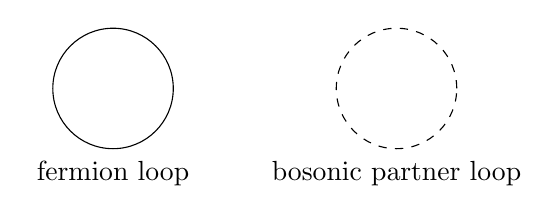
\begin{tikzpicture}[scale=0.9]
\draw (-2.0,0) circle (0.85);
\draw[dashed] (2.0,0) circle (0.85);
\node at (-2.0,-1.2) {fermion loop};
\node at (2.0,-1.2) {bosonic partner loop};
\end{tikzpicture}
\caption{Vergleich einer durchgezogenen mit einer gestrichelten Schleife im Argument zur Übereinstimmung der Ladungen. Die abgeschnittenen äußeren Markierungen werden nicht rekonstruiert, da sich aus dem Bild allein nicht alle Anbindungen bestimmen lassen.}
\end{figure}

\begin{classroomqa}
\audiencequestion{Könnten Superpartner der Entdeckung einfach deshalb entgangen sein, weil ihre Kopplungskonstanten verschieden sind? \lecturetimestamp{00:56:23}}
\lecturerresponse{Nicht, wenn sich dieselben Diagramme aufheben sollen. Durch das Hinzufügen von Photon-Wechselwirkungen wird die elektrische Ladung jeder Linie geprüft. Ungleiche Kopplungen führen zu ungleichen numerischen Schleifenfaktoren und lassen den großen Restbeitrag wieder auftreten. Die Symmetrie muss die entsprechenden Ladungen und Wechselwirkungen aufeinander abstimmen.}
\end{classroomqa}

\begin{classroomqa}
\audiencequestion{Müsste der Superpartner des Photons ebenfalls masselos sein? \lecturetimestamp{00:58:01}}
\lecturerresponse{In einer exakten supersymmetrischen Theorie wäre er masselos, weil er mit dem Photon entartet wäre. Die beobachtete Welt ist nicht exakt supersymmetrisch; daher muss ein physikalischer, photinoartiger Zustand nicht dieselbe Masse wie das Photon haben.}
\end{classroomqa}

\section{Das Wörterbuch der Superpartner}

Die Namensregeln sind nicht elegant, aber nützlich. Ein Boson erhält einen fermionischen Partner, dessen Name oft auf \emph{-ino} endet: Photon und Photino, das \(W\) und Wino, das \(Z\) und Zino, Gluon und Gluino, Higgs-Boson und Higgsino, Graviton und Gravitino. Ein gewöhnliches Fermion erhält einen bosonischen Partner, dessen Name meist mit \emph{s-} beginnt: Elektron und Selektron, Quark und Squark.

\begin{center}
\begin{tabular}{@{}>{\raggedright\arraybackslash}p{0.40\linewidth}>{\raggedright\arraybackslash}p{0.52\linewidth}@{}}
\toprule
gewöhnlicher Zustand & Superpartner und Spinänderung\\
\midrule
skalares Higgs-Boson, \(j=0\) & Higgsino, \(j=\tfrac12\); \(\Delta j=+\tfrac12\)\\
Eichboson, \(j=1\) & Gaugino, \(j=\tfrac12\); \(\Delta j=-\tfrac12\)\\
Materiefermion, \(j=\tfrac12\) & Sfermion, \(j=0\); \(\Delta j=-\tfrac12\)\\
Graviton, \(j=2\) & Gravitino, \(j=\tfrac32\); \(\Delta j=-\tfrac12\)\\
\bottomrule
\end{tabular}
\end{center}

Im Allgemeinen unterscheiden sich die Mitglieder eines Supermultipletts um eine halbe Einheit des Spins:
\begin{equation}
\Delta j=\frac12.
\end{equation}
In den groben Beispielen aus der Vorlesung ist ein Materiefermion mit Spin \(\tfrac12\) einem Skalar zugeordnet und ein Eichboson mit Spin eins einem Gaugino mit Spin \(\tfrac12\). In einem vollständigen wechselwirkenden Modell können sich die Zustände nach der Symmetriebrechung mischen; die physikalischen Masseneigenzustände müssen daher diese einfachsten Bezeichnungen nicht beibehalten.

\begin{classroomqa}
\audiencequestion{Könnten alle neuen skalaren Partner selbst eine spontane Symmetriebrechung durchlaufen? \lecturetimestamp{01:01:27}}
\lecturerresponse{Skalarfelder können Erwartungswerte annehmen, doch eine beliebige zusätzliche Symmetriebrechung wäre phänomenologisch verheerend. Ein realistisches supersymmetrisches Modell muss sein skalares Potential so gestalten, dass Farbe, elektrische Ladung und andere erforderliche Symmetrien nicht auf unerwünschte Weise gebrochen werden.}
\end{classroomqa}

\begin{classroomqa}
\audiencequestion{Hat das Higgsino besondere Wechselwirkungen, die dem quartischen Higgs-Term entsprechen? \lecturetimestamp{01:02:19}}
\lecturerresponse{Die Supersymmetrie stellt Beziehungen zwischen Wechselwirkungen ebenso wie zwischen Teilchen her. Diese Beziehungen ergeben sich nicht dadurch, dass man naiv jede Higgs-Linie durch eine Higgsino-Linie ersetzt; doch der skalare quartische Term und die zugehörigen fermionischen und Hilfsfeld-Wechselwirkungen gehören zu einer gemeinsamen, durch Bedingungen eingeschränkten Struktur. Diese Einzelheiten wurden in der Vorlesung noch nicht behandelt.}
\end{classroomqa}

\begin{classroomqa}
\audiencequestion{Gibt es Entsprechungen zum Drehungssatz für \(2\pi\) und \(4\pi\) in anderen Dimensionen? \lecturetimestamp{01:03:07}}
\lecturerresponse{Ja, doch die Dimensionalität verändert die Möglichkeiten. In zwei räumlichen Dimensionen können Austauschwege umeinander herumführen; dadurch sind Anyonen möglich, deren Austauschphasen allgemeiner sind als die bosonische Phase \(+1\) und die fermionische Phase \(-1\). Solche Anregungen treten in Festkörpersystemen auf, gehören aber nicht zum weiteren Verlauf dieser Vorlesung.}
\end{classroomqa}

\section{Warum exakte Supersymmetrie die Chemie auslöschen würde}

Wir fragen schließlich, wie eine Welt mit exakter Supersymmetrie aussähe. Exaktheit bedeutet hier gleiche Massen und aufeinander abgestimmte Wechselwirkungen für jedes Teilchen-Superpartner-Paar. Zum Elektron gäbe es ein bosonisches Selektron mit derselben Masse und elektrischen Ladung, und zum masselosen Photon ein masseloses fermionisches Photino:
\begin{equation}
m_{\widetilde e}=m_e,
\qquad
q_{\widetilde e}=q_e,
\qquad
m_{\widetilde\gamma}=m_\gamma=0.
\end{equation}

Die vertraute Periodizität der chemischen Elemente beruht auf der Fermi-Statistik. Wasserstoff hat ein Elektron in seinem niedrigsten Orbital. Helium kann dort zwei Elektronen unterbringen, weil sich ihre Spinbezeichnungen unterscheiden. Das dritte Elektron des Lithiums muss ein höheres Orbital besetzen: Das Pauli-Ausschlussprinzip verhindert, dass drei identische Elektronen denselben Einteilchenzustand einnehmen. Dieses äußere Elektron hat mehr Energie und würde bevorzugt nach innen fallen, wobei es gewöhnlich ein Photon aussendet; doch die besetzten tieferen Zustände blockieren den Übergang.

Exakte Supersymmetrie eröffnet einen weiteren Übergangskanal:
\begin{equation}
e^-_{\mathrm{outer}}
\longrightarrow
\widetilde e^-_{\mathrm{inner}}
+
\widetilde\gamma .
\end{equation}
Das anfängliche Elektron und das ausgesandte Photino sind Fermionen, während das verbleibende Selektron ein Boson ist. Da Selektronen der Bose- statt der Fermi-Statistik gehorchen, ist das Selektron im Endzustand nicht deshalb ausgeschlossen, weil sich bereits ein Teilchen im tiefer liegenden Orbital befindet. Das Valenzelektron kann sich daher umwandeln und nach innen fallen.

\begin{figure}[H]
\centering
\includegraphics[width=0.62\textwidth]{lecture_02_figure_06.png}
\lectureframe{01:09:18}

\medskip
\begin{tikzpicture}[scale=0.9]
\fill (0,0) circle (0.075);
\draw (0,0) circle (0.72);
\draw (0,0) circle (1.45);
\draw[-{Latex[length=2.2mm]}] (1.42,0.2) .. controls (1.2,0.52) and (0.92,0.42) .. (0.72,0.1);
\draw[decorate,decoration={snake,amplitude=1.4pt,segment length=7pt},-{Latex[length=2.2mm]}]
  (1.58,0) -- (3.55,0);
\node[above] at (2.7,0.12) {$\widetilde\gamma$};
\node[below] at (0,-1.65) {selectron drops to a lower orbital};
\end{tikzpicture}
\caption{Der atomare Übergang, der veranschaulicht, warum exakte Supersymmetrie die Chemie verändern würde. Die auslaufende Wellenlinie ist zu sehen; dass sie ein Photino darstellt, geht aus dem Transkript hervor.}
\end{figure}

Das betrifft nicht nur ein lithiumähnliches Atom. In einem großen Atom sorgen die Valenzelektronen für die chemische Vielfalt. Wenn sie sich wiederholt in bosonische Selektronen umwandeln können, können sie sich im energetisch niedrigsten verfügbaren Bereich anhäufen, statt Schalen aufzufüllen. Das Ergebnis wäre eine konzentrierte bosonische Population nahe dem Kern und nicht die vertraute Struktur der Valenzorbitale. Moleküle mit gerichteten Bindungen und teilweise gefüllten Schalen würden in ihrer bekannten Form nicht bestehen bleiben. Die Vorlesung nennt das hypothetische Lithium-Nachfolgeelement \emph{slithium}; der Scherz führt jedoch zu einer ernsten Schlussfolgerung: Exakte Supersymmetrie ergäbe Materie, die sich von gewöhnlicher Materie und damit auch von gewöhnlicher Biologie unterscheidet.

\begin{classroomqa}
\audiencequestion{Könnte die Kopplung des Übergangs vom Elektron zum Selektron so schwach sein, dass gewöhnliche Atome bestehen blieben? \lecturetimestamp{01:10:23}}
\lecturerresponse{Nicht in der hier betrachteten exakten Theorie. Die Supersymmetrie verknüpft den Übergang mit der elektromagnetischen Wechselwirkung, daher ist seine Kopplung durch die elektrische Ladung festgelegt und kann nicht frei beliebig klein gewählt werden. Die Vorlesung nennt für ein lithiumähnliches Atom eine grobe Lebensdauer in der Größenordnung einer Mikrosekunde. Das ist keine Präzisionsrechnung, sondern soll verdeutlichen, dass der Zerfall schnell wäre.}
\end{classroomqa}

Schon aus der Alltagsmaterie wissen wir also, unabhängig von Teilchenbeschleuniger-Experimenten, dass Supersymmetrie bei niedrigen Energien nicht exakt sein kann. Der Abstand zwischen den Massen von Teilchen und Superpartnern ist im Vergleich zu atomaren oder protonischen Skalen enorm, selbst wenn er im Vergleich zu einer Vereinheitlichungs- oder Planck-Skala winzig wäre.

\begin{classroomqa}
\audiencequestion{Warum ist die Supersymmetrie dann gebrochen? \lecturetimestamp{01:11:19}}
\lecturerresponse{Die Vorlesung bietet eine minimale Selektionsaussage: Wäre die Supersymmetrie nicht gebrochen, gäbe es keine Beobachter, die aus gewöhnlicher Chemie bestehen und diese Frage stellen könnten. Das ersetzt keine dynamische Theorie der Supersymmetriebrechung. Es erklärt lediglich, warum eine exakt supersymmetrische Welt bei niedrigen Energien nicht unsere Welt sein könnte.}
\end{classroomqa}

Supersymmetriebrechung ist mathematisch möglich und in vielen Konstruktionen recht generisch, doch eine realistische Brechung zu erreichen, ist keineswegs selbstverständlich. Umgekehrt haben exakt supersymmetrische Quantenfeldtheorien eine so besondere Struktur, dass sich manche von ihnen viel eingehender untersuchen lassen als generische Theorien. Sie dienen sowohl als mögliche Grundlage zur Ordnung der Teilchenphysik als auch als besonders leistungsfähige mathematische Laboratorien. In der nächsten Vorlesung geht es von dieser physikalischen Motivation ausgehend um weitere Aspekte dieser Struktur.

\section{Der Gedankengang}

Der Weg zur Supersymmetrie war bewusst indirekt angelegt:
\begin{enumerate}
\item Eine räumliche \(2\pi\)-Drehung gehört zu einer nichttrivialen topologischen Klasse, während sich eine \(4\pi\)-Drehung zur Identität deformieren lässt.
\item Unter einer \(2\pi\)-Drehung erhält ein Fermionzustand ein Minuszeichen; ein Experiment mit zwei Wegen macht dieses Vorzeichen beobachtbar, wenn es relativ statt global ist.
\item Aufgrund der Antisymmetrie von Fermionen beim Austausch erhält jede geschlossene Fermionschleife gegenüber einer Bosonschleife ein zusätzliches Minuszeichen.
\item Die entgegengesetzten Vorzeichen der Schleifenbeiträge ermöglichen symmetrieerzwungene Auslöschungen von Vakuum- und Skalar-Selbstenergiebeiträgen, wenn Massen und Kopplungen übereinstimmen.
\item Exakte Übereinstimmung gibt es in der Natur nicht. Wenn Supersymmetrie den Higgs-Sektor schützt, kann die Brechung die relevanten Partner nicht beliebig schwer machen.
\item Exakte Supersymmetrie bei niedrigen Energien würde es Elektronen ermöglichen, sich in bosonische Selektronen umzuwandeln und so die Schalenstruktur zusammenbrechen zu lassen, auf der die gewöhnliche Chemie beruht.
\end{enumerate}

Supersymmetrie ist also aus demselben Grund attraktiv und in ihrer naiv exakten Form unmöglich: Sie verknüpft Bosonen und Fermionen sehr eng. Diese enge Beziehung kann gefährliche Quantenkorrekturen eindämmen; bliebe sie jedoch bis in die Atomphysik hinein ungebrochen, sähe die Welt nicht mehr wie die uns vertraute aus.